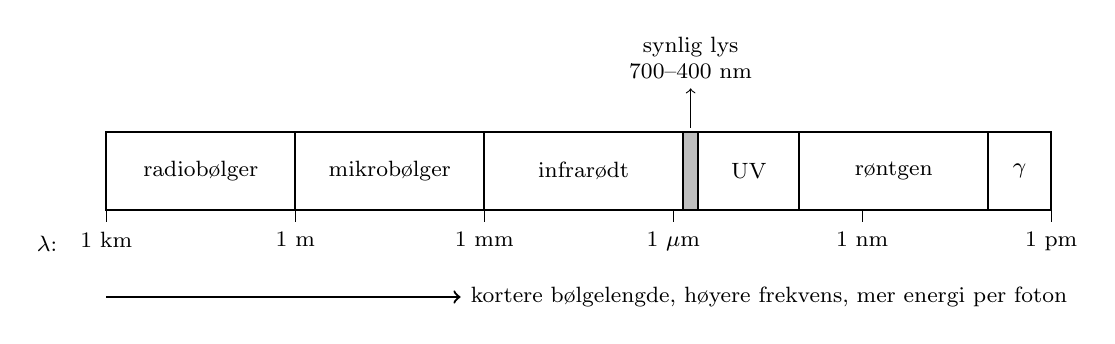
\begin{tikzpicture}[scale=1.0,font=\footnotesize]
\def\X#1{0.8*(3-#1)}
\foreach \a/\b/\t in {3/0/radiobølger, 0/-3/mikrobølger, -3/-6.155/infrarødt, -6.398/-8/UV, -8/-11/røntgen, -11/-12/$\gamma$} {
  \draw[thick] ({\X{\a}},0) rectangle ({\X{\b}},1);
  \node at ({(\X{\a}+\X{\b})/2},0.5) {\t};
}
\fill[black!25] ({\X{-6.155}},0) rectangle ({\X{-6.398}},1);
\draw[thick] ({\X{-6.155}},0) rectangle ({\X{-6.398}},1);
\draw[->] ({(\X{-6.155}+\X{-6.398})/2},1.05)--({(\X{-6.155}+\X{-6.398})/2},1.55) node[above,align=center]{synlig lys\\ 700--400 nm};
\foreach \e/\t in {3/1 km, 0/1 m, -3/1 mm, -6/1 $\mu$m, -9/1 nm, -12/1 pm} {
  \draw ({\X{\e}},0)--({\X{\e}},-0.15) node[below]{\t};
}
\node[left] at (-0.5,-0.42) {$\lambda$:};
\draw[->,thick] (0,-1.1)--(4.5,-1.1) node[right]{kortere bølgelengde, høyere frekvens, mer energi per foton};
\end{tikzpicture}
